\chapter{Introduction}
\section{Electronic Structure for Materials Science}
In 1987 Henry Ehrenreich published an article in Science called
``Electronic Theory for Materials Science"\cite{ehrenreich87}. The article begins
with a bold statement:

\begin{quote}
Theoretical Materials Science remains to be invented as a discipline, and for good reason.
\end{quote}

One of the reasons for this delayed maturity is that materials processing, 
historically, was a craft.

It will serve present purposes to consider what exactly constitutes a craft. 
There is some sense that the word craft in its common usage 
is to be distinguished from both science and art.
The word occupies a space somewhere between those two realms. 
A craft may bear an element of science in its application. 
The craftsman may possess a set of precision tools or 
established practices. However the process remains fundamentally shaped by 
the individual's choices. These choices are necessarily personal,
and it is in the course of making these choices that aspects 
of the craftsman's character is conferred to the final product. 

The rise of automation and mechanization means that the 
number of products bearing the mark of an individual craftsman's 
character is diminished. The mechanical homogeneity of the manufacturing process
become the distinguishing feature of the product. Where bespoke solutions are 
required one may still turn to the blacksmith and masons, who have the knowledge 
required to render from raw materials a composite product. In every case
whether individually or commercially manufactured it is the subtle
variations in the microstructure of a material which determines its 
strength, the way it reflects light, the way it conducts electricity, 
whether it flexes or snaps, whether it is hard or soft or magnetic.

In the realm of materials as craft we may take the example of Roman concrete.
%
Roman engineers learned to manufacture concrete from a 
particular mixture of volcanic sand called pozzolana,
taking its name from its point of extracion near Pozzuoli near Napoli. 
%
This pozzolana was mixed with quicklime, an aggregate, and seawater,
to produce a concrete of striking quality: 
particularly resistant to degradation in the presence of moisture.
This concrete was manufactured without any modern knowledge of microstructure 
and chemistry. Yet the people producing it must have been manipulating in their
mind some model of the underlying composition of the material and the effect of 
varying the proportions of the concretes constituents. 
%
%The pantheon today remains standing built with the same concrete poured centuries before.
%Is this true?
%
\footnote{For a description of Roman concrete and its use at the port at Pouzol see: Mariano Vasi, 
Itineraire Instructif de Rome à Naples, ou, Description Generale des Monumens Anciens et Modernes, 
Rome: [Mariano Vasi]. 1813, de Beer Itb 1815 V. For a broad perspective on metallurgical developments
see Paxton's article in Physics World \cite{paxton92}.} 

This concrete was manufactured without any modern knowledge of microstructure and 
chemistry.
%See a history of concrete and a history of energy
%\footnote{For a description of Roman concrete and its use at the port at Pouzol see: Mariano Vasi, 
%Itineraire Instructif de Rome à Naples, ou, Description Generale des Monumens Anciens et Modernes, 
%Rome: [Mariano Vasi]. 1813, de Beer Itb 1815 V.} 
%Though no doubt the engineers had some conception of what they were trying
%to accomplish and would have reasoned by analogy, an early application of
%Bohr's correspondence principle!
%Passing from the Romans to the middle ages we may encounter blacksmiths 
%who had over the centuries learned to manipulate the hardness of swords 
%and shields by controlling the alloying of metals and the 
%heat in the tempering process. 
%Again the theoretical model they worked with 
%lacked the modern conception of atomic composition 
%and microstructure.
%

Their expertise was developed based on part trial and error, 
part common sense, and part notion or, in a word, craft.

The underlying picture a theoretical materials scientist manipulates today
is a world composed of atoms interacting via electronic forces,
repelling each other when squeezed together, attracting each other at some
distance apart. 

\subsection{First Principles}
A comprehensive quantum theory describing the way atoms bind, the forces acting on them, 
the way electrons move through the solids, the way light interacts with electrons in solids
and the techniques to solve the equations governing these behaviours, has only 
arisen in the last 100 years. 
%
Over the past 40 years the combination of the theory and access to computers 
means the possibility of constructing accurate models of materials 
systems beginning from the arrangment of the constituent atoms has
progressed. 
%

This philosophy has given rise to the large field of ``first principles" or {\it ab initio}, 
(latin: from the beginning), modelling. 
%

The basic hypothesis of {\it ab initio} modelling is the following:  

\begin{quote}
Given the atomic numbers of a collection of atoms,
the number of electrons, and the arrangement of those atoms 
in space it is possible to compute
the expectation value of every experimental
observable of the system from that information.
\end{quote}

The philosophy bears a resemblance to the classical idea
that so long as the position and momentum of all particles 
is specified with arbitrary accuracy their subsequent 
trajectories could be predicted. 

Just as the classical ideas of complete mechanical determinism were
overthrown by the quantum theory I strongly suspect this
basic contention of {\it ab initio modelling} 
will be severely qualified itself. Fortunately, the 
state of {\it ab initio} modelling is such a long, long, way from being
able to predict observables from atomic position and number
in a truly non ad hoc fashion that this need not concern us. 
Only when that state has been attained
will some new ideas come along that mean 
we have to start all over again. It is to this end we strive.

The extent to which materials science has evolved to the point of being 
a truly 'first principles' theory is one of the themes of 
these notes \cite{finnis12, ismailbeigi2017}.
%
%Tracking the evolution of theoretical materials science may also allow 
%researchers to identify the avenues of research that are inefficient, 
%that are potentially obscuring knowledge, and convoluting 
%what is already understood. 
%
Ehrenreich's survey of the field from 30 years ago will provide the framework 
for charting the evolution of this field.
He identified four points that either characterized the state 
of the field of theoretical material science at the time or constituted essential principles 
that a satisfactory theory of materials must possess:
%
\begin{enumerate}[i)]
\label{en:ehrenreich}
\item Theory must be closely linked to experiment.
\item Ab initio calculations without approximations are virtually impossible 
      except in model systems.
\item Approximations are frequently based on prior experience rather 
      than on theoretical justification.
\item The study of trends in the properties of homologous materials 
      is a crucial ingredient of a credible theoretical framework.
\end{enumerate}
%
Unpacking the content of these four statements reveals where 
materials modelling has been successful, where it is lacking,
and what is required so that theoretical analysis becomes a driving
force in the development and manufacturing of novel materials.

\subsection{Scales of Materials Modelling}
What are the scales involved in materials modelling?
On what length scale is it important to treat the interactions
using quantum mechanics? What are the time scales? 
What is a typical number of particles?

To begin we consider the typical number of particles that are interacting.
Chemists arrived at the mol as a convenient unit for describing
quantities of atoms. A mol is on the order of $10^{23}$ atoms with
the precise number called the Avogadro Constant. While not strictly relevant
it is worth mentioning that Avogadro possesses one of the most
interesting scientific profile pictures. This picture is, quite rightly, reproduced
in a number of elementary chemistry books. We carry on this tradition 
in Fig.~\ref{fig:avogadro}.
%
\begin{figure}
\begin{center}
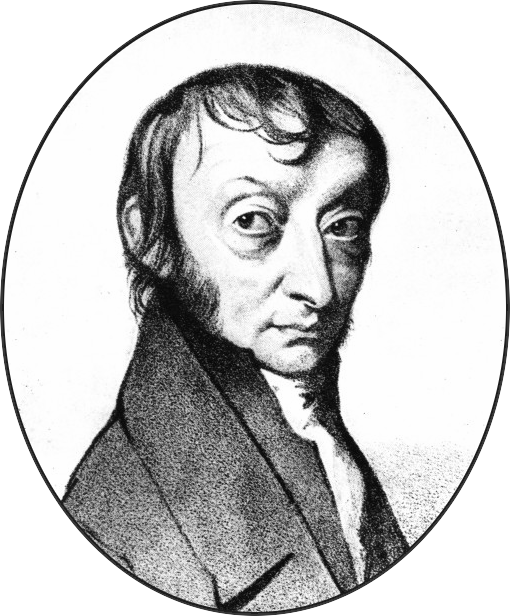
\includegraphics[scale=0.4]{./intro/Amadeo_Avogadro.png}
\end{center}
\caption{Count Amadeo Avogadro.}
\end{figure}
%
$10^{23}$ is by everyday standards an incredibly large number. 
It should go without saying, but often doesn't, that setting 
up a single system of equations to describe the motion of and mutual 
interactions of each individual particle in such an ensemble is not
a practical or meaningful endeavour, nor is it even necessary.
For such large aggregates of particles their mechanical behaviour seems 
well described by collective laws like ideal gas laws or continuum mechanics. 
So at what stage does it become necessary to describe the properties of the material
using quantum mechanics? 

In order to be more concrete about things let us consider a macroscopic specimen 
to be on the order of 200 nm$^{3}$ of material. A sample of material of this size 
is approaching the wavelength of visible light and could be
resolved with an optical microscope (using some focusing tricks). 
Assuming an atomic spacing of 2 tenths 
of a nanometer a dynamical simulation of around $10^{9}$ atoms 
done using quantum mechanics could be considered a quantum mechanical 
simulation of a macroscopic system. $10^{9}$, one billion, is a number
much more familiar than $10^{23}$.

To give an idea of the time required to perform such a simulation 
we may give an example of what, in the literature, would be considered 
a numerically well converged quantum simulation of sufficient accuracy. 
We will leave the notions of well-converged and accuracy intentionally vague
at this point suggesting only that were the results of this calculation
to be submitted to a referee they would not object outright to their
description as converged and accurate.

Simulating the forces on 250 quantum Fe atoms arranged in a particular crystal structure
required 4 hours of computing time on the local computing cluster (96 nodes).
There are 2000 electrons in the simulation which must be allowed
to rearrange themselves so they find their energetic minimum. 
%If computer technology continues developing at the same rate it has
%over the previous 30 years than within 60 years, with 
%no developements in the numerical techniques, 
%quantum mechanical simulations, to the same level 
%of accuracy, of millions of atoms should be feasible within a 
%similar amount of computing time. 

A single iteration of these equations will not provide us with 
much information. If it is desired to watch the collective 
motion of the atoms these calculations must be repeated with
the atomic positions updated according to the mechanical model chosen.
To resolve the vibrations of individual atoms  
time steps between iterations of a femtosecond, ($(10^{-15})$s),
are required. So every four hours of computing time yields $10^{15}$s
of atomic evolution.

To see the atoms do anything except complete a few oscillations around
their equilibrium position, i.e., if we wish to see something more interesting
in the simulation, like a dislocation
move through the crystal, a crack in the material begin to form, or
molecules adhered to a surface migrate and begin assembling something new,
would require thousands of femtoseconds, to arrive at a picosecond of data ($(10^{-12})$s).
For these sorts of computations we must reserve 5 months computing time on machine.
Another 12 orders of magnitude efficiency would remain to be found to 
simulate the motion of particles on time scales even approaching 
everyday experience.

These considerations are artificial for two important reasons. 
The first is I strongly suspect computational power will not continue 
developing at the rate seen over the previous 30 years. 
The second is that even if computational resources did continue growing 
at an equivalent rate; simulations of this nature would be of little value.

They would be of little value because were 
a simulation of this magnitude to be performed the
job of the theoretical material scientist would change. 
The task would now become the design of algorithms to identify 
processes of interest that occur within the data generated by 
these giant simulations. 
However, if the simulations are correct, these should correspond 
to the interesting processes observed in nature, which is why we wanted to
perform the simulations in the first place. We would be in the situation
of having done an enormous number of calculations at great computational
expense and we would be in exactly 
the same place we began. 

We would not have a theory that captures the mechanisms
underlying the behaviour of the system in a condensed mathematical notation. Nor 
would we would have an obvious way of inferring the likely experimental
observables for a homologous series of the material in question.

The objective of {\it ab initio} modeling is to extract meaningful information
about the essential parameters governing trends and characteristic properties 
of different classes of materials. Massive simulations generate such a quantity 
of data they can obscure reasoning and consume resources without providing insight 
and general principles. This observation stems directly from one of the
most fundamental tools for materials research: the periodic table. The 
organization of the table into groups and periods captures a huge range 
of phenomenon and possesses predictive power with little more computational
work than counting positive integers and a clever mode of tabulation.
The field of chemistry has made good use of that single table to guide
discovery and propose mechanisms.

Given that studying trends in homologous materials 
is a necessary component of a satisfactory
theory computer simulations have to be repeated 
over and over again, for every element in a group,
for each compound in a series, for each different structural conformation,
for differing alloy concentrations and so on. The ``one-off" character of 
numerical calculations makes them unsuitable as the basis for an actual 
theory of the measurable properties of homologous classes of materials.

There is another strange aspect to the properties of materials.
That is that many properties of materials can be described by a scalar, 
like Young's modulus, Poisson ratios, or small tensors to 
describe the elasticity. 
Electronic properties can be described using a single number 
like the dielectric constant of a material.
All these properties of systems are made up of many tiny degrees of freedom.
yet at some point all these variables merge into macroscopic parameters.
A satisfactory ab initio theory must capture this notion of {\it retraction on to} of
the multidimensional wavefunction in a many electron material onto easily manipulated
scalars or few indiced tensors.

It may sound as if computers are coming in for undue criticism. Not so! They
are the essential tool for theoretical materials science. What is being criticised
is the hypothetical user who would initiate a massive program of calculations without a
plan to harness the data generated so that the calculation need never be repeated.

Since Ehrenreich's article the development in computing hardware is easily charted. 
Clock speed, transistor density, storage, and the proliferation of high 
performance computing clusters with fast interconnects have greatly extended 
the range of problems that can be treated with numerical simulations
simply by providing more computational horse power.

Along with advances in hardware there have been a number
of methodological developments. These include compiler 
optimization, modern programming languages, 
shared libraries, object orientation, and stable open source 
platforms for code development, testing, and sharing. 

It is the important theoretical advances, i.e., the physical principles and
mathematical techniques that enable theoretical materials science 
which are more difficult to identify. It is difficult to identify what exactly 
the kernel of the theoretical idea is, and what precisely that idea has enabled. 

In the following sections, we describe in some more detail the 
actual scale of the increase in computing power and then we will
attempt to identify the major theoretical pillars of 
materials modelling.

\section{Digital Computation}
\label{sec:riseofcomp}
\begin{itemize}
\item Ab initio calculations without approximations are virtually impossible 
      except in model systems.
\end{itemize}

The second of Ehrenreich's points addresses the state of
{\it ab initio} calculations in 1988 and the inherent 
difficulties in performing them. The subsequent thirty years 
has seen an enormous extension of computing capacity. 
Before discussing the development of machines in the three decades since the 1980s it
is to worthwhile to reflect on the development of the machines in two
sets of three decades before the 1980s. 

%For an entertaing introduction to the history of computing see 
%George Dyson's Turing's Cathedral~\cite{dyson12} 
%and the references therein. For a technical review of 
%the state of computing in 1980 see Ref.~\cite{metropolis80}.

A suitable place to begin a potted history of $20^{\rm th}$
century computing is in 1936 with Alan Turing's, ``On Computable Numbers, 
With An Application to the Entsheidungsproblem"
\cite{turing36a}. Turing's concerns were in the domain of pure mathematics and
formal logic. However his method of tackling the problems in his chosen field by
invoking a black box machine capable of performing certain tasks by discrete operations,
would have transformative consequences for science and technology. 

Turing's hypothetical machine could advance and rewind a long,
segmented piece of tape one space to the left or one space to the right iteratively. 
The machine could print or erase a symbol on each segment of the tape and alter 
and maintain an internal state.
This abstract black box would serve as a computer and could be programmed 
to calculate. Turing made no formal engineering specifications for 
how that box should be built. 

The journey from this magic theory box to a machine capable of manipulating
numbers is the history of modern computing. From this basic set of processes
all the mechanisms to add, subtract, multiply, divide, take square roots, 
cubed roots, to take logs, to store, copy, and erase numbers, had to be 
invented. As Turing noted the important point about
these machines is that they are discrete, the fact that they are electronic
is an engineering choice; a choice made for speed.

A figure to set the scale for the rise in the accesibility of digitial computing 
in the 20$^{\rm th}$ century is given in a report
by the U.S. Office of Naval Research. Seventeen years after Turing's paper 
was published in March of 1953 there were 53 kilobytes of 
random access memory on Earth.\cite{dyson12, usonr53}
These kilobytes were scattered across a few private and government machines. 

One of the first major attempts to construct a physical computing machine was 
undertaken in Princeton. The machine was named \texttt{MANIAC} 
(Mathematical and Numerical Integrator and Computer).
The types of computations that were performed in the early days of the MANIAC 
were for thermonuclear applications. In an almost too perfect juxtaposition.
in the early hours of the night, between simulations of 
the shockwaves required to trigger thermonuclear explosions, Nils Baricelli 
would squeeze in the first computational biology simulations of how genes mutated
and combined to understand how living organisms might have emerged
and evolved. \cite{dyson12, barricelli54, barricelli62}.

The computational scientist of the early 1950s working
on the MANIAC had a number of additional 
technical difficulties to overcome beyond those of present day programmers. 
For instance programming errors, where reprogramming often meant physically rewiring
the machine, had to be surmounted along side exploding
vacuum tubes and mice meeting their untimely demise in the circuitry.

As the physical development of these machines progressed 
the algorithms that would be run on them had to be created.
One algorithm with which these notes will be particularly concerned was published by
Cornelius Lanczos: ``An Iteration Method for the Solution of the Eigenvalue Problem of Linear
Differential and Integral Operators"\cite{lanczos50}. In timely fashion, Lanczos described 
an iterative algorithm for determining the eigenvalues and eigenvectors for a given
matrix using a method particularly well suited to a computer. 
This iterative approach to determining the spectral properties of operators 
should become fairly familiar by the end of these notes. 
The algorithm itself and the way it is related to the computation
of material properties will be the first port of call in 
Chapter~\ref{eq:invariance}. 

Interestingly, for the purposes of our story, 
Cornelius Lanczos had also made an important contribution in the early
days of Quantum Mechanics. He was one of the early workers
to recognize the equivalence between the Schr\"odinger and Heisenberg
formulations of quantum mechanics\cite{lanczos26}. %see Zeitschrift fur Physik 35, 812 (1926). 
The means by which he related Heisenberg's matrix mechanics to
Schr\"odinger's wave equation was by exploiting a Green's function formalism. In addition
to the iterative approach to the solution of linear equations the use of Green's functions
will form a central topic of study in these notes. 

We now jump forward to 1987. The vacuum tubes have
now been replaced by solid state transistors. Our chosen 
representative from this era is the Connection Machine.
\footnote{One of the employees at Thinking Machines Corporation,
the company building the connection machine, was Richard Feynman
who would have been closely associated with those building and running
calculations in the 1950s. For an interesting discussion of the work they
did at Thinking Machines and Feynman's time there see W. Daniel
Hillis' article in Physics Today 42, 2, 78 (1989).}
%There was a strong focus on design at the company. Some of that
%work can be found at Tamiko Thiel's page}%; \url{http://www.tamikothiel.com/theory/cm_txts/di-frames.html}}

For those interested in such things we may list off specifications of 
that machine and compare them with a machine from 2017. The 
CM-2 was launched in 1987 and was configured with 512 MB of RAM and 25 GB of RAID
hard disk space. It had 65K microprocessors (each with 600 bytes of memory). 
By contrast the HPC machine presently accessible to the author 
is more easily measured in nodes. Each node in a machine has 2x12 core Intel Broadwell processors.
Each {\emph node} has 128 GB RAM and 120 GB static storage. The machine has in total 720 nodes. 
The processors themselves have up to 10 cores with clock speeds, the rate at which 
instructions can be executed, on the order of 3 GHz. A clock speed of 12.5 MHz 
would be representative in 1987. 
Each processor, on the `modern' machine, has a cache 
space of 10x 256 KiB L2 Cache, and 25 MiB of L3 cache,
this is to be compared with 600 bytes in the connection machine. 
Nowadays there could be on the order of 3 billion transistors in a 
single microprocessor; in 1987 that number would be closer to 100,000. 

Listing specifications like RAM and clock speeds doesn't necessarily clarify 
how much more powerful machines have become, 
but it is striking that in terms of speed, storage, and transistor density 
there are 3-5 orders of magnitude improvements in each category. 
The stability and optimization of compilers and the ease of programmability
of the machines has also improved.

A tour of the literature over the years reveals the changing nature of computation.
Perhaps the first ab initio determination of the electronic eigenvalues and eigenstates
in sodium using numerical techniques comes from a paper by von der Lage and Bethe in 1947:
%
\begin{quote}
In this connection the authors are indebted to Professor S. H. Caldwell of M.I.T. in making available the
use of the mechanical Bush Differential Analyzer; to Mr. P. O. Crawford who as a graduate assistant (1940)
made the work possible by operating the machine; to Dr. Martin Schwarzschild who ran an independent
check on two of the functions at the Thomas Watson Computing Bureau at Columbia University.
\end{quote}
%

%From C. A. Coulson from 1952 in a paper calculating the band structure of graphite, 
%``We should like to acknowledge the provision of a calculating machine by the
%British Iron and Steel Research Association..."

The ability to distribute and adapt code has also changed significantly. 
Code repositories, versioning systems, and the internet mean entire software
packages can be cloned, branched, modified, and shipped. We may compare the
present state of affairs with the following advertisement of an early version
of the Recursion Library (to be dealt with in detail soon):

\begin{quote}
C. M. M. Nex, Cambridge Recursion Method Library of computer
programs in FORTRAN, available from the Secretary, T.C.M. Group,
Cavendish Laboratory, Madingley Road, Cambridge CB3 0HE, England,
at a price of \pounds 5, \$ 10, or the equivalent to cover handling costs.
The library continues to be improved, the latest version
(November 1978) having been standardized to the same notation
as in the present volume.
\end{quote}

This constant and transforming development of computation that 
has played an important component in enabling {\it ab initio} 
calculations. 
It is this constant and dramatic development of computing capacity that 
means we may conclude that {\it ab initio} 
calculations are nowadays more routine then they when Ehrenreich was writing.
This constitutes an area of real progress in the field of theoretical
materials science. 

It would be unreasonable to hope 
the availability of computational resources will continue to develop
at the pace of the last thirty years. In these notes we will prefer to
consider ab initio calculations as having reached a satisfactory
plateau from which we can extract the essential data to build
the models that will underly our approach to theoretical
materials science.

\section{Computational Craft}
What sort of computations might a theoretical material scientist
wish to compute? One wish list has been provided by O.K. Andersen:
a material scientist may wish to:
\begin{quote}
... compute groundstate properties such as cohesive energies, interatomic forces, 
charge transfer, and magnetic moments, and also excitation spectra described 
by the one-electron Green's function\cite{anderson75}.
\end{quote}

The theoretical engines driving progress in numerical simulations of materials systems are
largely based on obtaining descriptions the electronic eigenstates 
of a system through mean field theories, the effective separation of core and 
valence electronic interactions to reduce the number of degrees of freedom, 
the choice of optimal basis sets for describing electronic states, 
and the various numerical algorithms for 
computing the eigenstates of electrons in material systems.

As a guide to which developments are considered important we may
use the citation metrics as a first approximation. The high level of 
activity in the field of materials science 
means that foundational papers number their citations in the tens of thousands. 

Table~\ref{tab:foundation} lists some of the papers in the field which, as
their citation count should imply, have enabled subsequent research. 
These techniques are divided into three categories, 
they are either theoretical justification for a calculation scheme, the description of
a technique that allows for more expedient and/or accurate calculations to be performed, 
or parameterizations of the exchange-correlation functional which permit the determination
of charge densities and electronic eigenvalues.

\begin{table}
\resizebox{\columnwidth}{!}{%
\begin{tabular}{|p{6cm}|l|p{6cm}|p{4cm}|}
\hline
Paper & Citations & Development & Category \\
Inhomogeneous Electron Gas \cite{hohenberg64} & 20,527 & Ground state energy of electron 
gas is universal functional of the density. & Theory \\
Self-Consistent Equations Including Exchange and Correlation Effects & 26,273 & Self-consistent 
set of equations for varying electron density. & Theory \\
New Method for Calculating the One-Particle Green's Function with 
Application to the Electron-Gas Problem & 2,599 & A calculation scheme for
obtaining progressively more accurate approximations to the 
one-electron Green's function. \cite{hedin65} & Theory \\
Linear methods in band theory \cite{andersen75}& 4,822 & Describes LAPW and LMTO 
approach to electronic structure calculations. & Theory/Implementation \\
Electron correlation in semiconductors and insulators: Band gaps and 
quasiparticle energies \cite{hybertsen86} & 1,929 & Extension of electronic structure 
calculations to excited states. & Theory/Implementation \\
\hline
\end{tabular}}
\caption{Citations are relevant up to Nov. 2017. Citations are according 
to the journals in which they appear. 
The actual number of citations are much higher. 
\label{tab:theoreticalpapers}}
\end{table}

There are no doubt many valid criticisms of Table~\ref{tab:foundation}.
One obvious criticism is that it is biased towards a particular approach to electronic structure
based on the description of electronic states using plane waves, pseudopotentials, and density
functional theory. These methods are suitable for crystalline systems with periodicity and can be pushed 
to describe more disordered systems on the order, as discussed in Sec.\ref{sec:riseofcomp}, 
of one thousand atoms. These sorts of techniques are also often favoured by workers 
studying metallurgical systems from first principles and materials with potential 
electronic applications.

%To broadly categorize the workers we can say a material scientist 
%is interested in crystals, alloys, ceramics, glasses, and, possibly, rubbers and elastomers. 
%Chemists are interested in molecules, 
%tend to use localized basis sets and exploit Monte Carlo and 
%related methods to obtain energy bounds on the order of a few meV. 
%For a pedagogical presentation of the connection between band 
%theory and the chemist's molecular orbital picture 
%see Ref.~\cite{hoffman87}. Physicists are interested in lasers, 
%Ising and Hubbard models, and the general positions of resonances 
%and asymptotes in very cold materials and won't be discussed further. 

\section{Justification by Utility}
The observation that materials processing has evolved in the manner 
of a craft has been imitated in the development of the 
theory of materials science. Much of first principles modelling is reliant on
the realization that certain approximations work well. The first is 
the separatation of degrees of freedom. That is that some electrons in a solid are
tightly bound to a nucleus and behave similarly to how they might behave in an atom.
This allows these "core electrons" to be frozen out of a calculation, 
via some transformation, and only valence electrons need to be considered. 
This is an important realization in chemistry as well where it has 
been long recognized that chemical trends are dominated by
the valence electrons of atoms. Accordingly, chemical elements are 
grouped together in the table by their valency. 

\begin{table}
\resizebox{\columnwidth}{!}{%
\begin{tabular}{|p{6cm}|l|p{6cm}|p{4cm}|}
\hline
Paper & Citations & Development & Category\\
\hline
Norm-Conserving Pseudopotentials \cite{hamann79} & 2,156 & Nodeless eigenfunctions 
that match atomic eigenvalues. & Pseudopotentials \\
Soft self-consistent pseudopotentials in a generalized 
eigenvalue formalism \cite{vanderbilt90} & 11,560 & Effective pseudopotentials for 
first row and transition-metal systems. & Pseudopotentials \\
Projector augmented-wave method \cite{blochl94paw} & 19,194 & Generalizes pseudopotential 
and LAPW methods; allows reconstruction of wavefunctions at nucleus. & Pseudopotentials \\
Efficacious Form for Model Pseudopotentials \cite{kleinman82} & 3,709 & Reduces number of 
integrals which need to be calculated in pseudopotential calculations. & Pseudopotentials \\
Unified Approach for Molecular Dynamics and Density-Functional Theory \cite{car85} & 5,940 & Combined 
molecular dynamics and density functional theory. & Theory/Implementation \\
High-precision sampling for Brillouin-zone integration in metals \cite{methfessel89} & 2,908 & Brillouin 
zone integration. & Numerical Integration Technique \\
Improved tetrahedron method for Brillouin-zone integrations \cite{blochl94} &  2,986 & Brillouin zone 
integration. & Numerical Integration Technique\\
Special points for Brillouin-zone integrations \cite{monkhorst76} & 21,361 & Brillouin zone 
integration. & Numerical Integration \\
\hline
\end{tabular}
}
\caption{Citations are relevant up to Nov. 2017. Citations are according to the journals 
in which they appear, the actual number of citations are much higher. These selections 
have been chosen as representative of the important theoretical and algorithmic developments
which have enabled subsequent research. In some cases there are a number of contemporary papers which
treat the same problems but failed to "catch on", or describe techniques which differ 
in an incremental way to the works cited here. \label{tab:foundation}}
\end{table}

\subsection{Exchange and Correlation}
Without wishing to get bogged down in the technical details of Chapter~\ref{chap:manybodygw}
we will only remark that to obtain a description of the electronic states of material requires
a reasonable description of how the electrons in a material interact. Electrons interact
with each other via the Coulomb potential which is simple enough. However the long range of 
this potential, the singularities when the electrons overlap and the difficulty of evaluating
matrix elements of a many body wavefunction with the coulomb potential have motivated alternative
approach to incorporating the effect of the interaction of the electrons in material.
If we look at the work done based on parameterization of the exchange correlation functional 
we see the number of citations approaches 100,000.
%Naturally that figure includes significant 
%double counting of citing work, on the other hand we have not included cross citations 
%between journals in many of the figures quoted, so with some lucky 
%cancellation the number is probably representative. 

The parameterization is based on what may be considered an abstract question,
``What might happen if we start squeezing electrons into an imaginary box?".
We have moved from Turing's computing box to an imaginary box of electrons
which has been pondered for close to a century now. In passing 
we observe that the practical utility of these speculative 
boxes is unreasonable. 

One outcome of the box of electrons is a family of 
unremarkable curves that describe the relationship between
the density of electrons in the box and a total energy. 

The practical consequence is this curve enables the
structural, electronic, and vibrational properties of an 
enormous class of materials to be calculated with creditable accuracy.
%
\begin{table}
\resizebox{\columnwidth}{!}{%
\begin{tabular}{|p{6cm}|l|p{6cm}|p{4cm}|}
\hline
Paper & Citations & Development & Category\\
\hline
Ground State of the Electron Gas by a Stochastic Method \cite{ceperley80} & 8,855 & Calculation of the 
exchange-correlation energy of an electron gas. & Exchange Correlation \\
Atoms, molecules, solids, and surfaces: Applications of the generalized gradient approximation 
for exchange and correlation \cite{perdew92} & 11,418 & Incorporates information from the 
gradient of the density. & Exchange Correlation \\
Self-interaction correction to density-functional approximations 
for many-electron systems \cite{perdew81} & 11,629 & Parameterization of Ceperley-Alder 
data on free electron gas. & Exchange Correlation \\
Accurate and simple analytic representation of the electron-gas 
correlation energy \cite{perdew91} & 12,296 & Parameterization of exchange 
correlation functional. & Exchange Correlation \\
A new mixing of Hartree–Fock and local density‐functional 
theories \cite{becke93} & 7,143 & Combining Hartree-Fock and DFT. & Exchange Correlation \\
Generalized Gradient Approximation Made Simple \cite{perdew96} & 47,029 & GGA functionals 
improved.& Exchange Correlation \\
\hline
\end{tabular}
}
\caption{Citations are relevant up to Nov. 2017. Citations are according to the journals 
in which they appear, the actual number of
citations are much higher. These selections have been chosen as representative of the 
important theoretical and algorithmic developments
which have enabled subsequent research. In some cases there are a number of 
contemporary papers which treat the same problems but failed to "catch on", 
or describe techniques which differ in an incremental way to the works cited here. 
\label{tab:foundation}}
\end{table}
%
Just how creditable this approach is returns again to point three. 
The theoretical justifications for the success of the approach are
secondary to the fact that prior and ongoing experience suggests 
these techniques capture the quantitative and qualitative features
of experimental observation. The rate of their acceptance 
and adoption seems to have tracked their usage in a positive 
feedback loop. 

If you look through a typical density functional based electronic structure code 
it is interesting to look at the routine responsible for calculating 
the local exchange correlation potential. 
The input required is the electronic density at a point in space \footnote{Beyond the local density
approximation there a range of increasingly complex parameterizations and
approximations to the exchange-correlation functional. For instance some functionals
require the gradient of the density at a point in space.} 
This  density is inserted as the argument of a subroutine and a single number is returned
representing an energy. The curve as a function of density 
has little more structure than that given in Fig.~\ref{fig:ldapz}. 
%
\begin{figure}
\begin{center}
\graphicspath{{./intro/}}% GNUPLOT: LaTeX picture with Postscript
\begingroup
  \makeatletter
  \providecommand\color[2][]{%
    \GenericError{(gnuplot) \space\space\space\@spaces}{%
      Package color not loaded in conjunction with
      terminal option `colourtext'%
    }{See the gnuplot documentation for explanation.%
    }{Either use 'blacktext' in gnuplot or load the package
      color.sty in LaTeX.}%
    \renewcommand\color[2][]{}%
  }%
  \providecommand\includegraphics[2][]{%
    \GenericError{(gnuplot) \space\space\space\@spaces}{%
      Package graphicx or graphics not loaded%
    }{See the gnuplot documentation for explanation.%
    }{The gnuplot epslatex terminal needs graphicx.sty or graphics.sty.}%
    \renewcommand\includegraphics[2][]{}%
  }%
  \providecommand\rotatebox[2]{#2}%
  \@ifundefined{ifGPcolor}{%
    \newif\ifGPcolor
    \GPcolortrue
  }{}%
  \@ifundefined{ifGPblacktext}{%
    \newif\ifGPblacktext
    \GPblacktextfalse
  }{}%
  % define a \g@addto@macro without @ in the name:
  \let\gplgaddtomacro\g@addto@macro
  % define empty templates for all commands taking text:
  \gdef\gplbacktext{}%
  \gdef\gplfronttext{}%
  \makeatother
  \ifGPblacktext
    % no textcolor at all
    \def\colorrgb#1{}%
    \def\colorgray#1{}%
  \else
    % gray or color?
    \ifGPcolor
      \def\colorrgb#1{\color[rgb]{#1}}%
      \def\colorgray#1{\color[gray]{#1}}%
      \expandafter\def\csname LTw\endcsname{\color{white}}%
      \expandafter\def\csname LTb\endcsname{\color{black}}%
      \expandafter\def\csname LTa\endcsname{\color{black}}%
      \expandafter\def\csname LT0\endcsname{\color[rgb]{1,0,0}}%
      \expandafter\def\csname LT1\endcsname{\color[rgb]{0,1,0}}%
      \expandafter\def\csname LT2\endcsname{\color[rgb]{0,0,1}}%
      \expandafter\def\csname LT3\endcsname{\color[rgb]{1,0,1}}%
      \expandafter\def\csname LT4\endcsname{\color[rgb]{0,1,1}}%
      \expandafter\def\csname LT5\endcsname{\color[rgb]{1,1,0}}%
      \expandafter\def\csname LT6\endcsname{\color[rgb]{0,0,0}}%
      \expandafter\def\csname LT7\endcsname{\color[rgb]{1,0.3,0}}%
      \expandafter\def\csname LT8\endcsname{\color[rgb]{0.5,0.5,0.5}}%
    \else
      % gray
      \def\colorrgb#1{\color{black}}%
      \def\colorgray#1{\color[gray]{#1}}%
      \expandafter\def\csname LTw\endcsname{\color{white}}%
      \expandafter\def\csname LTb\endcsname{\color{black}}%
      \expandafter\def\csname LTa\endcsname{\color{black}}%
      \expandafter\def\csname LT0\endcsname{\color{black}}%
      \expandafter\def\csname LT1\endcsname{\color{black}}%
      \expandafter\def\csname LT2\endcsname{\color{black}}%
      \expandafter\def\csname LT3\endcsname{\color{black}}%
      \expandafter\def\csname LT4\endcsname{\color{black}}%
      \expandafter\def\csname LT5\endcsname{\color{black}}%
      \expandafter\def\csname LT6\endcsname{\color{black}}%
      \expandafter\def\csname LT7\endcsname{\color{black}}%
      \expandafter\def\csname LT8\endcsname{\color{black}}%
    \fi
  \fi
    \setlength{\unitlength}{0.0500bp}%
    \ifx\gptboxheight\undefined%
      \newlength{\gptboxheight}%
      \newlength{\gptboxwidth}%
      \newsavebox{\gptboxtext}%
    \fi%
    \setlength{\fboxrule}{0.5pt}%
    \setlength{\fboxsep}{1pt}%
\begin{picture}(5760.00,3960.00)%
    \gplgaddtomacro\gplbacktext{%
      \csname LTb\endcsname%%
      \put(1078,2420){\makebox(0,0)[r]{\strut{}$-0.1$}}%
      \put(1078,2684){\makebox(0,0)[r]{\strut{}$-0.08$}}%
      \put(1078,2948){\makebox(0,0)[r]{\strut{}$-0.06$}}%
      \put(1078,3211){\makebox(0,0)[r]{\strut{}$-0.04$}}%
      \put(1078,3475){\makebox(0,0)[r]{\strut{}$-0.02$}}%
      \put(1078,3739){\makebox(0,0)[r]{\strut{}$0$}}%
      \put(1210,2200){\makebox(0,0){\strut{}$0$}}%
      \put(2041,2200){\makebox(0,0){\strut{}$0.2$}}%
      \put(2871,2200){\makebox(0,0){\strut{}$0.4$}}%
      \put(3702,2200){\makebox(0,0){\strut{}$0.6$}}%
      \put(4532,2200){\makebox(0,0){\strut{}$0.8$}}%
      \put(5363,2200){\makebox(0,0){\strut{}$1$}}%
    }%
    \gplgaddtomacro\gplfronttext{%
      \csname LTb\endcsname%%
      \put(198,3079){\rotatebox{-270}{\makebox(0,0){\strut{}Energy (Ry.)}}}%
      \csname LTb\endcsname%%
      \put(4376,3566){\makebox(0,0)[r]{\strut{}PZ Correlation Energy}}%
    }%
    \gplgaddtomacro\gplbacktext{%
      \csname LTb\endcsname%%
      \put(946,704){\makebox(0,0)[r]{\strut{}$-1$}}%
      \put(946,915){\makebox(0,0)[r]{\strut{}$-0.8$}}%
      \put(946,1126){\makebox(0,0)[r]{\strut{}$-0.6$}}%
      \put(946,1338){\makebox(0,0)[r]{\strut{}$-0.4$}}%
      \put(946,1549){\makebox(0,0)[r]{\strut{}$-0.2$}}%
      \put(946,1760){\makebox(0,0)[r]{\strut{}$0$}}%
      \put(1078,484){\makebox(0,0){\strut{}$0$}}%
      \put(1935,484){\makebox(0,0){\strut{}$0.2$}}%
      \put(2792,484){\makebox(0,0){\strut{}$0.4$}}%
      \put(3649,484){\makebox(0,0){\strut{}$0.6$}}%
      \put(4506,484){\makebox(0,0){\strut{}$0.8$}}%
      \put(5363,484){\makebox(0,0){\strut{}$1$}}%
    }%
    \gplgaddtomacro\gplfronttext{%
      \csname LTb\endcsname%%
      \put(198,1232){\rotatebox{-270}{\makebox(0,0){\strut{}Energy (Ry.)}}}%
      \put(3220,154){\makebox(0,0){\strut{}$\rho$ (e/a.u.$^{3}$)}}%
      \csname LTb\endcsname%%
      \put(4376,1587){\makebox(0,0)[r]{\strut{}PZ Exchange Energy}}%
    }%
    \gplbacktext
    \put(0,0){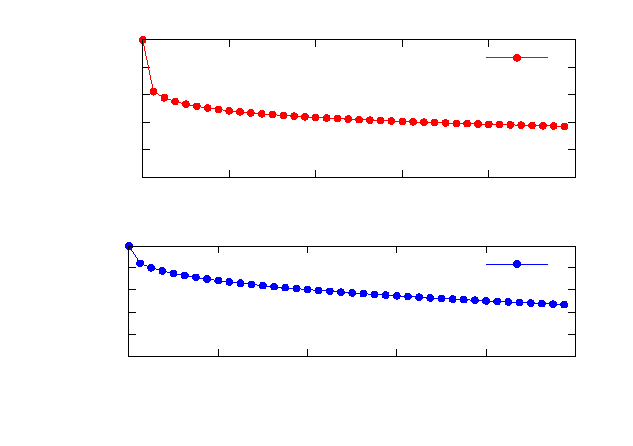
\includegraphics{pz}}%
    \gplfronttext
  \end{picture}%
\endgroup

\caption{Perdew-Zunger parameterization of the correlation and exchange energies 
for an electron gas. This curve and those like it enable a great deal of 
contemporary materials modelling. For reference
a crystal of iron would have an electronic density of 
around 0.36 e/a.u.$^{3}$ (electrons per cubic
atomic unit). A silicon crystal would have an electronic density in the 
range of 0.02 e/a.u.$^{3}$, carbon in the diamond conformation 
would be around 0.1 e/a.u.$^{-3}$.  
\label{fig:ldapz}.}
\end{center}
\end{figure}
%
Curves of this type have been used to perform calculations and simulations for 
materials composed of elements from across the periodic table. They have been
used to compute all the properties of interest, cohesive energies, magnetic moments, 
band gaps, etc. with varying degrees of success.

%Despite its apparent simplicity, in all manner of crystalline systems, 
%this functional enables the theoretical
%prediction of accurate ground state properties and structures entirely from first principles. 
There are trends at the moment to reparameterize the simplest exchange-correlation functional
in order that simulations return a better description of experimental data. The extent
to which this reparameterization is helpful is debateable. 
Part of the appeal of the simplest local density approximations is that it is universal. 
Where a calculation fails to reproduce an experimental data point, and this failure is 
attributed to the exchange correlation functional, it will be argued that 
applying a more sophisticated treatment of exchange and correlation is 
preferred to introducing a complicated reparameterization of the exchange correlation
function itself.

\begin{figure}
\includegraphics[scale=0.35]{./intro/TimelineLocaltoGlobal.png}
\caption{A selection of papers from 1980 to 1992 that representative of two differing schools of thought. 
Above the line, global methods based on total energy functionals and large scale computing, below the 
line local models of interatomic forces and structures. The two approaches are complementary.}
\end{figure}

%\section{The Cross-Over}
%A component of the thesis which inspired these notes is 
%that there was at some point a crossover where local semi-empirical
%models of condensed matter systems was over taken by {\it ab initio} 
%calculations based on density functional theory. 
%Heralded in Finnis \cite{andersen89}  with reference to \cite{payne87}.
%The ubiquity of access to {\it ab initio} data has had a significant impact on 
%Ehrenreich's first point: experimental corroboration. 
%Cursory surveys of the literature demonstrate the increasing frequency of 
%appearance of publications which contain no original experimental work. 

Ehrenreich's four points clarify the desired objective for materials modelling:
a minimal theoretical model informed by {\it ab initio} calculations that accounts for 
experimental data, and {\it predicts quantitatively} trends in material properties
across homologous series. In these notes the possibility of exploiting the invariance theorem 
and recursion techniques is assessed as the optimal framework
for achieving this objective. 

\section{Prospective}
The purpose of these notes is to collect established tools into 
a framework for mapping first principles knowledge about material systems 
onto concise mathematical models. 

In the first chapter the ideas underlying invariance and the 
theory of the local atomic environment are presented along with references
to the original work. The recursion technique is introduced. 
Recursion techniques are viewed as the {\emph central unifying technique} in these
notes and all subsequent discussion is formulated with recursion in mind.

After having spent some (considerable) time on invariance and recursion
Chap.~\ref{chap:gw} makes the standard presentation of Density Functional Theory along 
with a brief discussion of the Harris-Foulkes functional and tight-binding theory. 
Density Functional Theory is the primary {\it ab initio} engine that will 
provide the interaction parameters required in recursion formulations.
Alongside the standard DFT presentation in Chapter~\ref{chap:gw} we will
introduce a more advanced treatment for the correlation of electrons in materials.
This is called, ominously, and (to the uninitiated) confusingly, $GW$ theory.

Chapter~\ref{chap:wannier} is a whistle stop tour 
on modern techniques for preparing localized wave packets in the 
form of Wannier functions. The focus of this chapter is on 
ways of deducing the coefficients of a sparse Hamiltonian
appropriate for performing recursion type calculations.

%Perhaps the most ambitious objective is to couple
%quantum-mechanical modeling of small, critical regions of a 
%system (such as a dislocation core) with a less rigorous modeling
%of the noncritical regions ( which could be modeled using
%classical elasticity theory). \cite{payne92}

%We will then discuss the outlines of an idea for 
%including many-body corrections to the standard 
%single particle formulation of recursion theory. 
%This perturbation theory is especially important for electronic 
%applications where bands gaps and excitation energies 
%are the most important quantities. It is also essential for
%energy level alignment at all sorts of interfaces. In fact the range
%of applications is so great they will be left to a separate set of notes
%only the broad ideas will be discussed here.

%Chapter~\ref{chap:superconductivity} is devoted to
%certain aspect of the theory of superconductivity. 
%This is related to recursion theory by sketching some ideas for 
%local computations of the screened Coulomb and electron-phonon
%coupling parameters required to compute transition temperatures.

Chapter~\ref{chap:metallurgy} looks at metallurgical concepts 
and a few interesting calculations which can be performed 
using recursion techniques. 

Finally, Chapter \ref{chap:bayes} extends recursion techniques
to the regime of macroscopic mechanical properties 
and points out some Bayesian techniques 
for selecting material models and ranking them according 
to a mathematical criterion. 
%Married with recursive techniques
%it is possible to identify novel atomistic configurations
%and extend our knowledge of materials system by "learning on the fly" 
%in the sense it was intended by Alessandro De Vita.

All of these techniques have been developed by other workers 
over a number of years. Collecting them into a single place 
and working through some applications still seems a worthwhile 
endeavour. 

As a companion to these notes a version of Chris Nex's and 
Roger Haydock's Cambridge Recursion Library
has been imbedded in a python library. A number of practical examples 
of calculations can be worked through using this library and these 
exercises are indicated throughout the notes. 
This companion calculator's value lies not only
in the numbers it provides but the physical insight afforded by the 
calculations. This valuable computational package can then be used for 
whatever calculations one desires.

The recursion method placed in the broad context of twentieth century 
condensed matter physics is admittedly niche. It has its practitioners, 
its uses, its successes and limitations like any other field.
However to the author its importance lies in the close connection between the mathematical
technique and the reality it seeks to describe. That is the way 
an electron may be associated with 
one atom and then, through its excursions, hopping from atom to atom as it explores 
it environment, forming new combinations. It is this process which
generates the braids and chains which link atoms together into new structures 
with new properties.

%From Adrian's biographical sketch of Friedel
% Could only think about crystals in reciprocal space
% `owing to an overdose of X-ray scattering.'

%Gibb's has suggested that:
%
%\begin{quote}
%One of the principal objects of theoretical research is to
%find the point of view from which the subject appears in its
%greatest simplicity.
%\end{quote}

This complementarity of mathematical technique and physical reality 
is best articulated by Heisenberg in a tribute to his friend Rudolf Peierls:
 
\begin{quote}
In the case of theoretical physics, as we learned it primarily from
Bohr, the essence neither consists of proofs
nor in the mathematical description of experiments.
Rather the convincing power of the mathematics employed comes from
what one calls physical insight or physical interpretation. The supreme
requirement of this type of physics is to understand every formula that
one writes down physically both as to its intellectual content and to its context.
\end{quote}
 
It is hoped the close marriage of physical insight and mathematical technique 
afforded by the recursion method will point to a framework where engineers, informed by the
structure, connectivity, and composition of a material, can consult a simple table of
coefficients and directly perform their computations, perhaps even with 
pen and paper. The result of these computations should yield accurate 
properties of their system derived from quantum mechanics.
Properties like band gaps, elasticity tensors, conductivities, 
heat capacities, cohesive energies, adhesive energies, superconducting transition temperatures, 
and so on. Such a framework would constitute a useful calculus for quantum engineers.
